\chapter{应用筛选框架\mytool}
\label{chp:fakerevealer}

\mytool 是由Python 3开发的一个仿冒应用筛选框架,由应用收集器、迭代搜索器和仿冒应用过滤器三个组件组成,\autoref{fig:FakeRevealer}展示了\mytool 的整体流程图。
通过正版APK为输入,\mytool 在经过迭代搜索、样本下载、仿冒应用过滤三个步骤之后,将以CSV文件和JSON文件的形式输出仿冒应用各数据项和拓展后的正版应用信息。

\begin{figure}[htbp]
	\centering
	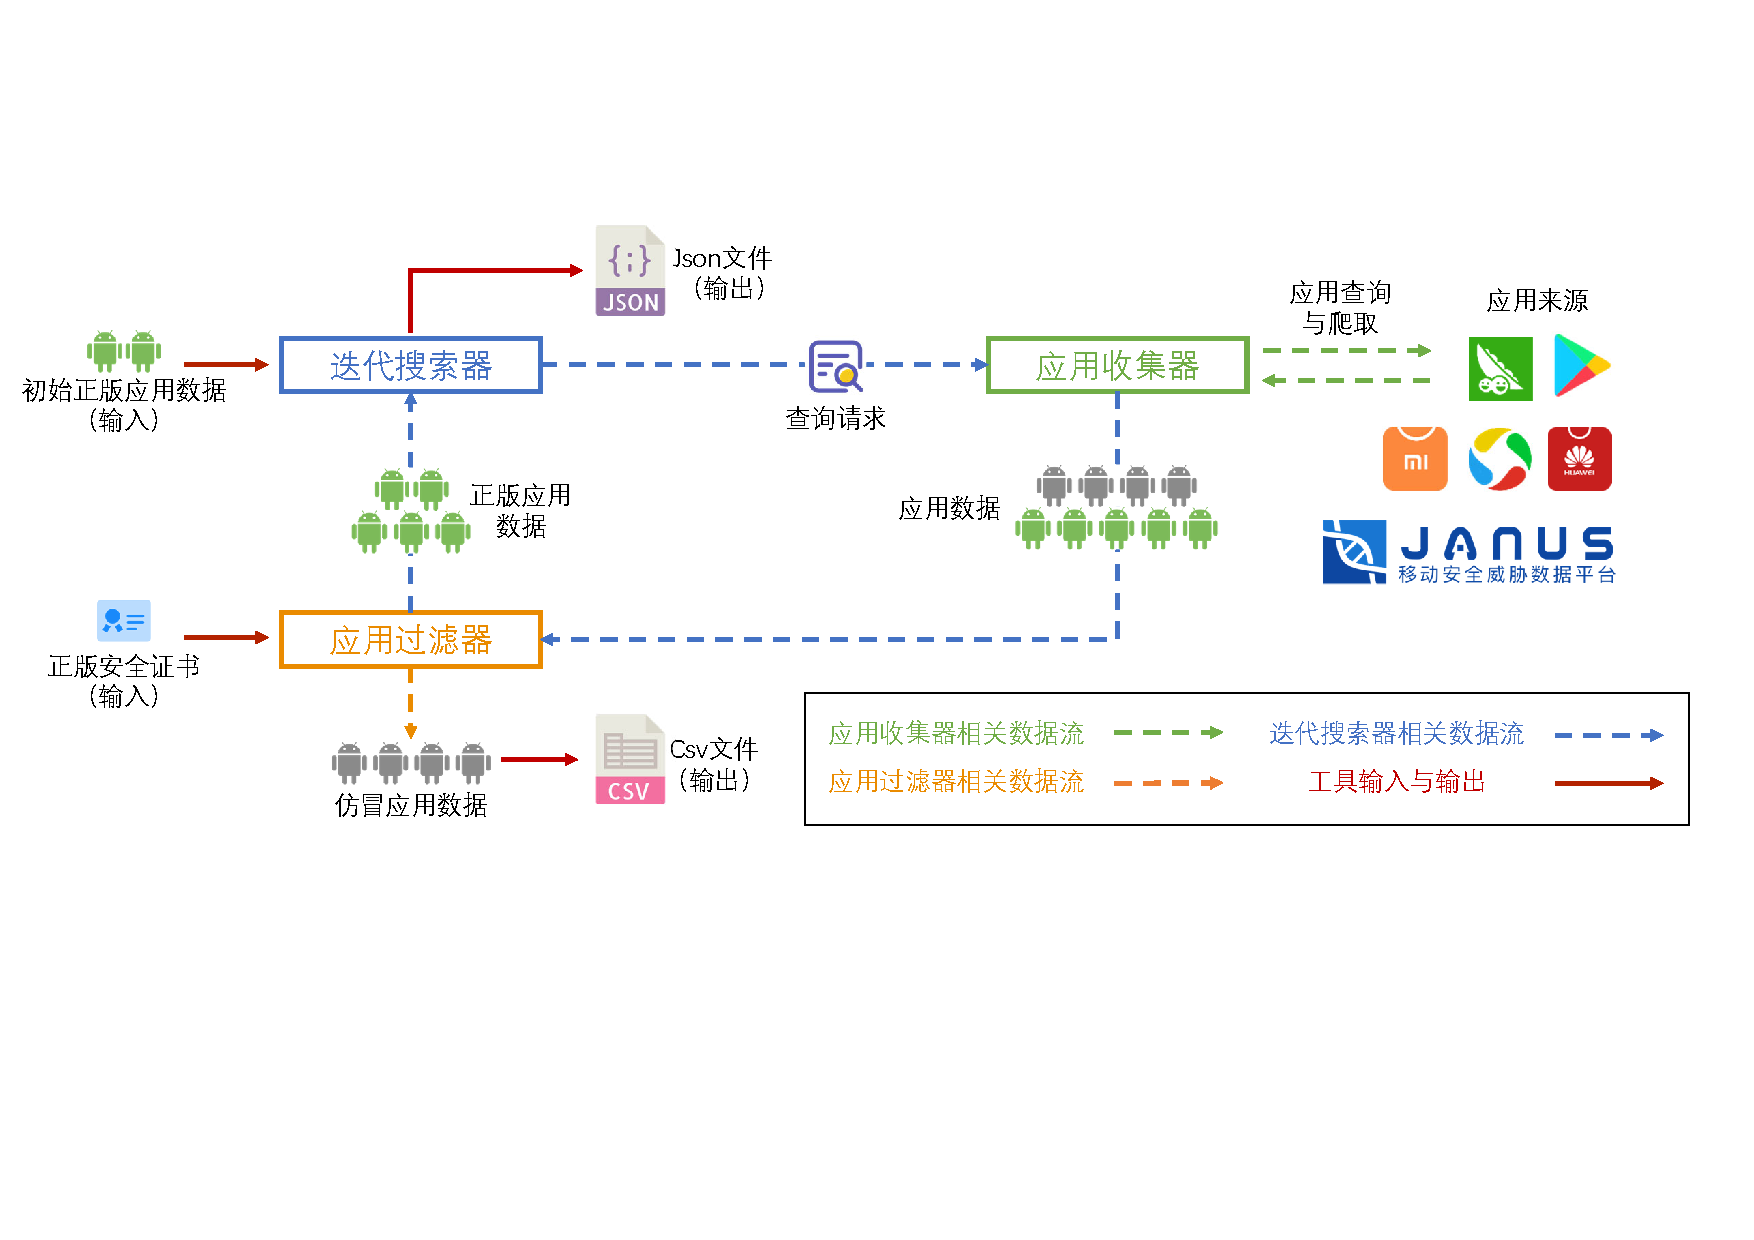
\includegraphics[width=0.95\textwidth]{./Figures/edwin-fakerevealer}
	\caption{\mytool 整体结构}
	\label{fig:FakeRevealer}
	\vspace{-3mm}
\end{figure}


\section{组件设计与实现}


\subsection{应用收集器}
应用收集器是与应用来源直接交互的部分,分为两个不同的子模块,分别是网络爬虫模块和APK包预处理模块。
在接收到应用收集请求之后,应用收集器会先根据收集请求,利用网络爬虫模块下载应用,然后再用APK包预处理模块对下载完毕的APK包提取信息,方便后续操作。

1)\ \emph{网络爬虫模块} \quad
本模块负责接收应用收集器的输入,根据输入中的需求从应用来源中查询并下载对应的App。
由于Janus平台上已经有提前收集好的源于各个应用市场的App样本,我们可以直接从Janus上爬取应用。

实际上,虽然应用商店提供应用查询、下载的API不同,不存在可以对应所有应用市场的爬虫脚本,但只要能分析出这些API的名称和用法,结合应用商店账户的Cookies,我们也能从商店中下载应用。
考虑到这个方面,我们开发了插件化的爬虫模块。
针对不同的应用商店,我们可以在使用网络包分析工具(如Burpsuite~\cite{burpsuite})解析到API与Cookies信息之后,将对应API和Cookies写入配置插件,再对网络爬虫模块配置对应当前商店的插件,开始爬取应用。

在具体实现方面,我们利用Python自带的urllib库实现对网络资源的访问;由于下载是可以并发进行的事务,为了能提高运行效率,我们利用了threading库对网络爬虫模块提供了多线程特性。

2)\ \emph{APK包预处理模块} \quad
这个模块负责从下载完毕的APK包中提取指定的数据项,存入键值对中,最后将所有应用的数据键值对以列表形式返回,作为应用收集器的输出。
APK文件中虽然包含着应用的所有信息,但我们的应用筛选并不需要用到整个APK文件,所以我们可以把筛选需要用到的数据先提取出来,后续处理时直接调用与该APK包有关的数据即可。
同时,由于不同APK包的大小不一,所需下载时长也各异,我们利用了较大的应用还在下载的时间,对已经下载完毕的APK提取信息。
比起让应用收集器直接返回下载完毕的APK包、待后续需要数据时再进行数据提取的方法,这样的设计可以减小内存占用,也提高了框架的运行效率。

具体实现方面,APK包预处理模块使用Python的os库实现对命令行指令的调用,然后利用Android SDK中自带的命令行工具aapt对APK包进行解析,获取指定的数据项。


\subsection{迭代搜索器}
这个模块的设计利用了基于一个BFS的算法,详情可见\autoref{alg:bfs}。
根据已有的正版应用信息,本组件向应用收集器提交查询、下载样本的请求,然后利用仿冒应用过滤器过滤获得的应用信息,再根据其中正版应用的数据扩增正版应用信息,进行下一轮迭代搜索。

\begin{algorithm}[!ht]
	\tablewuhao
	\caption{迭代搜索算法}
	\label{alg:bfs}
    \KwIn{ $targetItems$,列表,用于拓展的数据项}
    \KwIn{ $legalApkInfo$,列表,包含正版应用及其信息键值对}
	\KwOut{ $searched$,列表,包含拓展后的正版应用信息键值对}
	\SetKwProg{Fn}{Function}{:}{}

	\Fn {iterSearcher($legalApkInfo, targetItems$)} {

        $wtQueue$ = $\emptyset$;

        $searched$ = $\emptyset$;

        \For {$apkInfo \in legalApkInfo$} {

            \For {$item \in targetItems$} {

                $wtQueue$.add(${item: apkInfo[item]}$);

            }

        }

    	\While {$wtQueue \ne \emptyset$} {

    		$key, val$ = $wtQueue$.pop();

    		\If{${key: val} \in searched$} {continue;}

    		$searched$.add(${key: val}$);

    		$newSamples \gets$ appRetriever($key, val$);

    		\For {$sample \in newSamples$} {

                $isLegal \gets $ FakeFilter($sample$).getResult();

    			\If {$isLegal$} {

    				$sampleInfo \gets sample$.getInfo();

    				\For {$item \in targetItems$} {

    					$wtQueue$.add(${item: sampleInfo[item]}$);

    				}

    			}

    		}

    	}

    \KwRet{$searched$};

    }

\end{algorithm}

\autoref{alg:bfs}的输入有两项,分别是已有的正版应用信息列表$legalAppInfo$和要用来拓展搜索范围的数据项$targetItems$。

算法开始前,我们先遍历每个正版应用的信息,将要拓展搜索的数据项对应的内容$apkInfo[item]$插入到待查询队列$wtQueue$中,完成初始化(第4 - 6行)。
然后我们开始迭代搜索应用。
每次迭代中,我们都从$wtQueue$中取出一组键值对,其中键$key$为本次迭代中用于搜索新应用的数据项,$val$为数据项对应的值(第8行)。
取出键值对之后,我们先检查该键值对是否已经被用于之前的搜索中。
如果该键值对之前已经出现过,那么我们跳过本轮迭代,重新取一组键值对进行搜索;
否则,我们将本组键值对放入集合$searched$,表示该组键值对已被使用过。
之后,我们将键值对传递给应用收集器,应用收集器会生成对应查询,从应用来源中获取数据项相关的应用(第12行)。
对于应用收集器返回的应用集$newSamples$中的每个样本$sample$,我们会用仿冒应用过滤器检查$sample$是否为正版样本。
如果是正版样本,那么我们将从该样本中获取对应的数据$sampleInfo$,然后将其中与待拓展对应项$item$对应的内容插入到待查询队列$wtQueue$中(第15 - 18行)。
当应用集$newSamples$中的所有样本都被筛选检查过之后,本轮迭代结束。
如果$wtQueue$中的所有键值对都已经被检索完毕(即$wtQueue$为空),本算法流程结束,本组件会将$searched$中被用于拓展搜索的各个数据项键值对整理成JSON文件输出,方便之后的再利用。

在本次实证研究场景中,$targetItems$包含两项内容,一个是应用的包名(\emph{PackageName}),另一个是应用自身的名字(\emph{AppName})。
之所以要这样操作,是因为开发者推出的App的应用名和包名并不是一成不变的。
一些热门应用会出于商业原因频繁地更改自己的应用名(比如爱奇艺视频,会根据其近期热播的电视剧/电影变更其应用名以吸引更多用户使用);
也有个别的热门应用可能会更换自己的包名,比如App有重大改版、又或者是开发者安全证书有变更,开发者不得不更换包名(具体原因可参考\secref{sec:signature}的Android App签名机制部分)。

\subsection{仿冒应用过滤器}
顾名思义,仿冒应用过滤器的功能是从输入的应用程序集之中将仿冒应用筛选出来,其核心是安全证书的识别。
根据\secref{sec:signature}中对Android应用签名机制的描述,一个App中包含的安全证书文件指示了对APK文件进行修改的开发者。
如果一个APK文件中包含的安全证书信息与指定应用的开发者信息相符,那么我们相信这个APK包来源于正版的开发者;否则我们认为这是一个仿冒应用。

在开始过滤之前,开发者需要先向过滤器输入正版APK文件,以导入正版证书信息。
之后,对于每个输入的应用,我们会将其安全证书信息和正版证书信息作比对。
对于证书信息相符的应用,我们会将其放入迭代搜索器的待检索队列中用作下一轮的迭代搜索;
而证书信息不相符的应用则会被筛选出并保存。

在迭代搜索的流程结束之后,本组件会将保存的所有仿冒应用数据项导出成CSV文件保存,方便之后的数据挖掘。

\section{本章小结}
本章讲述了应用过滤系统\mytool 的工作流程,以及其中三个组件——应用收集器、迭代搜索器和仿冒应用过滤器的设计实现。
尽管\mytool 在设计之时选择了利用包名和应用名迭代搜索、通过安全证书筛选的机制过滤仿冒应用,但框架本身的流程并不囿于此机制中,读者可以参考本框架流程,设计其他过滤仿冒应用,或者是其他任何具有某种特征的应用的工具。

在明确数据收集流程之后,我们将针对仿冒样本中采集到的元数据进行数据挖掘,以求获得对于仿冒应用生态和特征、以及对于仿冒应用开发者的行为的更全面的认知。
